% Options for packages loaded elsewhere
\PassOptionsToPackage{unicode}{hyperref}
\PassOptionsToPackage{hyphens}{url}
%
\documentclass[
]{article}
\title{Predicting Rainfall in Australia}
\author{Jannick Akkermans (1727324)}
\date{17-12-2021}

\usepackage{amsmath,amssymb}
\usepackage{lmodern}
\usepackage{iftex}
\ifPDFTeX
  \usepackage[T1]{fontenc}
  \usepackage[utf8]{inputenc}
  \usepackage{textcomp} % provide euro and other symbols
\else % if luatex or xetex
  \usepackage{unicode-math}
  \defaultfontfeatures{Scale=MatchLowercase}
  \defaultfontfeatures[\rmfamily]{Ligatures=TeX,Scale=1}
\fi
% Use upquote if available, for straight quotes in verbatim environments
\IfFileExists{upquote.sty}{\usepackage{upquote}}{}
\IfFileExists{microtype.sty}{% use microtype if available
  \usepackage[]{microtype}
  \UseMicrotypeSet[protrusion]{basicmath} % disable protrusion for tt fonts
}{}
\makeatletter
\@ifundefined{KOMAClassName}{% if non-KOMA class
  \IfFileExists{parskip.sty}{%
    \usepackage{parskip}
  }{% else
    \setlength{\parindent}{0pt}
    \setlength{\parskip}{6pt plus 2pt minus 1pt}}
}{% if KOMA class
  \KOMAoptions{parskip=half}}
\makeatother
\usepackage{xcolor}
\IfFileExists{xurl.sty}{\usepackage{xurl}}{} % add URL line breaks if available
\IfFileExists{bookmark.sty}{\usepackage{bookmark}}{\usepackage{hyperref}}
\hypersetup{
  pdftitle={Predicting Rainfall in Australia},
  pdfauthor={Jannick Akkermans (1727324)},
  hidelinks,
  pdfcreator={LaTeX via pandoc}}
\urlstyle{same} % disable monospaced font for URLs
\usepackage[margin=1in]{geometry}
\usepackage{longtable,booktabs,array}
\usepackage{calc} % for calculating minipage widths
% Correct order of tables after \paragraph or \subparagraph
\usepackage{etoolbox}
\makeatletter
\patchcmd\longtable{\par}{\if@noskipsec\mbox{}\fi\par}{}{}
\makeatother
% Allow footnotes in longtable head/foot
\IfFileExists{footnotehyper.sty}{\usepackage{footnotehyper}}{\usepackage{footnote}}
\makesavenoteenv{longtable}
\usepackage{graphicx}
\makeatletter
\def\maxwidth{\ifdim\Gin@nat@width>\linewidth\linewidth\else\Gin@nat@width\fi}
\def\maxheight{\ifdim\Gin@nat@height>\textheight\textheight\else\Gin@nat@height\fi}
\makeatother
% Scale images if necessary, so that they will not overflow the page
% margins by default, and it is still possible to overwrite the defaults
% using explicit options in \includegraphics[width, height, ...]{}
\setkeys{Gin}{width=\maxwidth,height=\maxheight,keepaspectratio}
% Set default figure placement to htbp
\makeatletter
\def\fps@figure{htbp}
\makeatother
\setlength{\emergencystretch}{3em} % prevent overfull lines
\providecommand{\tightlist}{%
  \setlength{\itemsep}{0pt}\setlength{\parskip}{0pt}}
\setcounter{secnumdepth}{-\maxdimen} % remove section numbering
\newlength{\cslhangindent}
\setlength{\cslhangindent}{1.5em}
\newlength{\csllabelwidth}
\setlength{\csllabelwidth}{3em}
\newlength{\cslentryspacingunit} % times entry-spacing
\setlength{\cslentryspacingunit}{\parskip}
\newenvironment{CSLReferences}[2] % #1 hanging-ident, #2 entry spacing
 {% don't indent paragraphs
  \setlength{\parindent}{0pt}
  % turn on hanging indent if param 1 is 1
  \ifodd #1
  \let\oldpar\par
  \def\par{\hangindent=\cslhangindent\oldpar}
  \fi
  % set entry spacing
  \setlength{\parskip}{#2\cslentryspacingunit}
 }%
 {}
\usepackage{calc}
\newcommand{\CSLBlock}[1]{#1\hfill\break}
\newcommand{\CSLLeftMargin}[1]{\parbox[t]{\csllabelwidth}{#1}}
\newcommand{\CSLRightInline}[1]{\parbox[t]{\linewidth - \csllabelwidth}{#1}\break}
\newcommand{\CSLIndent}[1]{\hspace{\cslhangindent}#1}
\usepackage{subfig}
\ifLuaTeX
  \usepackage{selnolig}  % disable illegal ligatures
\fi

\begin{document}
\maketitle

\hypertarget{introduction}{%
\subsection{1. Introduction}\label{introduction}}

Rainfall is a common event that happens in every country. The amount of
rain that falls on a given day can depend on several factors. For
example, one would expect that if the temperature is high enough, water
will evaporate. This evaporated water then cools down when it is far
away from the surface. Because of this cooldown, the water transitions
from a gaseous phase into a liquid phase, creating clouds containing
water. The water subsequently becomes too heavy for the clouds to carry,
resulting in rainfall. The temperature depends in its turn on the
climate. Take Australia for example. Summers in Australia can become
quite warm, with an average temperature of 29 degrees Celsius. Another
factor that could influence rainfall is windspeed. With a high wind
speed, it is expected that clouds fly by quicker which lowers the
rainfall in a certain region. When combined with the dry climate, it is
essential to make good predictions about the rainfall so that good
precautionary measures can be taken. Therefore, the research question of
this report will be: ``What are useful predictors of the rainfall in
Australia?'' I expect that wind speed would be a useful predictor for
the reason mentioned before. I also expect that the maximum temperature
is a useful predictor of rainfall since Nicholls, Drosdowsky, and Lavery
(1997) found a negative correlation between the maximum temperature and
rainfall in Australia. Finally, I believe that the minimum temperature
will be a useful predictor as well since Nicholls, Drosdowsky, and
Lavery (1997) also found a positive correlation between the minimum
temperature and rainfall in Australia.

The dataset that will be used to answer the research question is derived
from the site Kaggle, which hosts many publicly available datasets that
can be used for many projects. The dataset I downloaded from Kaggle
contains data about the climate in Australia. Some of the variables used
in this dataset are for example the maximum temperature on a given day,
the rainfall on that day, and the wind direction on that day. For this
project, I will only use the minimum temperature, the maximum
temperature, the wind speed, and the amount of rainfall to answer the
research question previously addressed. When initially inspecting the
dataset, it came to my attention that there are some missing values
present in the dataset. Therefore, I decided to impute those missing
values to obtain a complete dataset. A complete dataset can potentially
provide more information for the question at hand.

To impute the missing values, the MICE algorithm (van Buuren and
Groothuis-Oudshoorn (2011)) will be used. This algorithm creates five
possible datasets in which the missing data are imputed from the
available data. This is done five times, thus creating 25 possible
datasets. All these datasets are subsequently pooled to create a final
dataset in which the missing values are now replaced by a pooled
estimate of the 25 possible datasets. Subsequently, the variables
MinTemp, MaxTemp, and WindGustSpeed are centered so that they contain a
useful, interpretable zero point when the regression estimates are
evaluated later in this project. Finally, I will sample 2000
observations from the original dataset. The reason for this is because
the original dataset is quite large, which could lead to memory
problems. Additionally, working with a smaller sample generally speeds
up the overall project.

\hypertarget{estimation}{%
\subsection{2. Estimation}\label{estimation}}

To answer the research question addressed in the previous section, the
possible predictors have to be estimated. The estimation will take place
using the Bayesian approach, which utilizes prior knowledge about the
parameters of interest and the data at hand. It combines the prior
knowledge and the density of the data into a joint posterior
distribution. This joint posterior distribution is subsequently used to
sample for example 1000 values for the parameters of interest. With
these sampled values, Bayesian statistics like the Expected A Posteriori
(EAP) and the 95\% Central Credible Interval (CCI) can be calculated.
The 95\% CCI will give me an indication of the relevance of the
predictors. As I said earlier, the joint posterior distribution is
derived by combining the density of the data and prior knowledge about
the parameters of interest. This can be done exactly based on the prior
distribution and the density of the data using Bayes' theorem. However,
one can also approximate the posterior distribution using Markov-Chain
Monte Carlo (MCMC) algorithms, for example, the Gibbs sampler. The Gibbs
sampler derives conditional posterior distributions for each of the
parameters of interest and uses those to approximate the joint posterior
distribution. To derive the conditional posterior distributions for the
predictors in this project, I need to specify the density of the data
and the prior distributions for each of the predictors. The density of
the data can be described with the following regression equation:

\begin{align}
  rainfall_i = b_0 + b_{1}X_{1i} + ... + b_{n}X_{ni}
\end{align}

This means that the density of the data is a normal distribution with as
mean \(b_0 + b_{1}X_{1i} + ... + b_{n}X_{ni}\) and as variance
\(\sigma^2\). As for the prior, it is typical to use conjugate priors
which have the same form as the resulting conditional posterior
distribution. For the predictors MaxTemp (centered, from now on called
MaxTemp.cen) and MinTemp (centered, from now on called MinTemp.cen), I
will use a normal conjugate prior. Since I do not have any historical
data that investigated the same question and I am not certain about the
relationship between maximum temperature and rainfall, I will use an
\(X \sim \mathcal{N}(0,0.0001)\) uninformative prior. The variance of
the density of the data is sampled using the normal density and an
inverse-gamma prior. I also decided to use an uninformative prior for
the conditional posterior of the variance. For the predictor
WindGustSpeed (centered, from now on called WindGustSpeed.cen), I
decided not to use the same prior as for the predictors MinTemp.cen and
MaxTemp.cen. The reason for this is that I am less certain that there is
a relationship between wind gust speed and rainfall. Therefore, I use a
non-standardized t-distribution as prior distribution to allow for more
uncertainty. The non-standardized t-distribution is not a conjugate
prior, which means that it will not lead to a closed-form conditional
posterior distribution. In such cases, one uses the Metropolis-Hastings
(MH) sampler which is described in the next section.

\hypertarget{metropolis-hastings}{%
\subsection{3. Metropolis-Hastings}\label{metropolis-hastings}}

As described before, I use a non-standardized t-distribution as prior
distribution for the variable WindGustSpeed.cen with a normal density of
the data. Since the density and the prior distribution are not of the
same form, the resulting conditional posterior will not be of a
recognizable form. Therefore, I will use a Metropolis-Hastings (MH)
sampler to draw samples for the variable WindGustSpeed.cen.
Metropolis-Hastings works by deriving functions proportional to the
conditional posterior and using those to approximate the joint posterior
distribution. The reason that MH is more suitable here than Gibbs is
that knowing the distribution up to a proportionality constant is enough
to sample from it using MH. Therefore, it does not matter that the final
conditional posterior can not be found. In this project, I multiply the
t-distribution prior with the normal density and use the resulting
proportional function in the MH sampler.

The Metropolis-Hastings sampler works as follows: first, it samples a
candidate value from a proposal distribution. The type of proposal
distribution depends on the type of MH sampler that is used. In an
independent MH sampler, a candidate value is drawn from a proposal
distribution with the same parameters in each iteration. The proposal
distribution does not depend on the previous value of the parameter of
interest, hence the term independent. In a dependent MH sampler, the
parameters of the proposal distribution depend on the previous value of
the parameter of interest. Therefore, there is more flexibility in the
values that can be drawn from it. In this project, I will use a random
walk MH sampler with a normal proposal distribution whose mean is the
current value of the parameter of interest. Next, a ratio between the
candidate value as a function of the proportional function and the
current value as a function of the proportional function is calculated.
This ratio is then multiplied with a ratio between the current value of
the parameter of interest and the candidate value. The latter ratio is
implemented so that the Metropolis-Hastings algorithm does not tend to
get stuck at a certain value. When these two ratios are multiplied with
each other, the resulting acceptance ratio is compared to a threshold
value sampled from a uniform distribution ranging from 0 to 1. If the
acceptance ratio is equal to or higher than the threshold value, the
candidate value is accepted as the new current value. If the acceptance
ratio is lower than the threshold value, the candidate value is rejected
and the current value is assigned as the accepted value in that
iteration. Since the values of a certain parameter using the MH sampler
are based on accepting or rejecting the candidate value, the quality of
the proposal distribution can be examined with an acceptance ratio. The
quality can also be analyzed by calculating the autocorrelation which
will be explained in section 6.

\hypertarget{model-selection-using-the-dic}{%
\subsection{4. Model selection using the
DIC}\label{model-selection-using-the-dic}}

Now that the density of the data and the densities and priors for the
predictors have been specified, multiple models can be compared to find
the best fitting model to the data in this project. When the best
fitting model has been found, I can evaluate the parameter estimates to
answer the research question. In this project, I will compare 3
competing models with each other. The first model contains MaxTemp.cen
and WindGustSpeed.cen as predictors of Rainfall. The second model tries
to predict Rainfall from MinTemp.cen and WindGustSpeed.cen. The third
and final model has Rainfall predicted by MaxTemp.cen, MinTemp.cen, and
an interaction between these predictors. The reason for the inclusion of
the interaction is that {[}1{]} found a positive correlation between
maximum temperature and minimum temperature. Therefore, I believe the
interaction between maximum and minimum temperature to be a possible
predictor. The different competing models are compared to each other
using the Deviance Information Criterion (DIC). The DIC is based on
minimizing the `loss' or `deviance,' which is defined as the distance
between a model of interest and a saturated model (i.e.~a model that
fits the data perfectly). Mathematically, the DIC is formulated as
follows:

\begin{align}
  DIC = -2 log f(y|\theta) + 2pD
\end{align}

where \(log f(y|\theta)\) is the loglikelihood of the model of interest
evaluated at the means of the regression parameters and where \(pD\) is
defined as the estimated number of `effective parameters.' The estimated
number of effective parameters is calculated with

\begin{align}
  pD = Dbar - Dhat 
\end{align}

where \(Dhat\) is the loglikelihood previously described and where
\(Dbar\) is the mean of the loglikelihoods of the imposed model
evaluated at each set of sampled regression parameters. Using the DIC,
the best fitting model can be selected. Usually, a difference in DIC
larger than 10 means the model with the higher DIC can be ruled out. A
difference between 5 and 10 can also be seen as a substantive
difference, thus allowing for the selection of the model with the lower
DIC. The first model achieved a DIC of 13345, the second model a DIC of
13340. This means there is a DIC difference of 5, meaning that the
second model fits the data substantively better than the first model.
Next, the second model is compared to the third model. The third model
achieved a DIC of 13288. This means there is a difference of 52 between
the third and second model. Since this is much larger than 10, I can
safely reject the second model and select the third model as the
best-fitting model.

\hypertarget{model-selection-using-the-bayes-factor}{%
\subsection{5. Model selection using the Bayes
Factor}\label{model-selection-using-the-bayes-factor}}

A good fitting model for the data in this project can also be found by
using the Bayes Factor (BF). The Bayes Factor is typically used to test
informative hypotheses (e.g.~\(b_1\) \textgreater{} \(b_2\)) against
uninformative hypotheses (e.g.~\(b_1\) = \(b_2\)) or to test informative
hypotheses (e.g.~\(b_1\) \textgreater{} \(b_2\)) against their
complement (e.g.~\(b_1\) \textless= \(b_2\)). The BF is calculated by
dividing the fit of the specified hypothesis by the complexity of that
hypothesis. The complexity of a hypothesis is defined as the proportion
of the prior distribution that is in concordance with the specified
hypothesis (Hoijtink et al. (2019)). The fit of a hypothesis is defined
as the proportion of the posterior distribution that is in concordance
with the specified hypothesis (Hoijtink et al. (2019)). The resulting BF
value indicates how many more times there is evidence for a specified
hypothesis than for its complement or the uninformative hypothesis.
Although there are no guidelines for determining when there is enough
evidence for a given hypothesis, numbers greater than 1 typically
indicate that the specified hypothesis would hold. Using the Bayes
Factor, three hypotheses are compared to determine which predictors
should be included in the final model. The data for MaxTemp.cen are
multiplied by -1 for these comparisons to allow for a better comparison
of the effect of MaxTemp.cen with the effects of any other predictors.
The hypotheses are evaluated using the bain() package in R.

The first hypothesis, H1, is defined as follows:

\begin{align*}
H_1: b_1 > b_2
\end{align*}

where \(b_1\) is the regression coefficient of MaxTemp.cen and \(b_2\)
is the regression coefficient of WindGustSpeed.cen. The BF for this
hypothesis tested against its complement is 5.44, meaning there is 5.44
times more evidence for H1 than for its complement. Therefore, I would
conclude that MaxTemp.cen is a useful predictor to include in the final
model.

The second hypothesis, H2, is defined as

\begin{align*}
H_2: b_3 > b_2
\end{align*}

where \(b_3\) is the regression coefficient of MinTemp.cen and \(b_2\)
still the regression coefficient of WindGustSpeed.cen. The BF for this
hypothesis tested against its complement is 6.57, meaning there is 6.57
times more evidence for H2 than for its complement. This leads me to
conclude that MinTemp.cen is also a useful predictor for the final
model.

The final hypothesis, H3, is defined as

\begin{align*}
H_3: b_4 > b_1*b_3
\end{align*}

where \(b_4\) is the regression coefficient for the interaction between
MaxTemp.cen and MinTemp.cen, \(b_1\) the regression coefficient of
MaxTemp.cen and \(b_3\) the regression coefficient of MinTemp.cen. The
BF for this hypothesis tested against its complement is 34.71, meaning
there is 34.71 times for evidence for H3 than for its complement.
Therefore, the interaction between MaxTemp.cen and MinTemp.cen should
also be included in the final model. Ultimately, all the included
parameters using the Bayes Factor lead to the same model as the model
selected through the DIC. Therefore, the final model that will be
evaluated consists of the predictors MaxTemp.cen, MinTemp.cen and an
interaction between these predictors.

\hypertarget{convergence}{%
\subsection{6. Convergence}\label{convergence}}

To arrive at reliable estimates of the regression coefficients, one
wants to have sampled as many different values as possible from the
approximated joint posterior distribution. This means that one wants the
model to have converged so that the model has covered as much from the
joint posterior distribution as possible. Convergence can be assessed in
four ways and is typically checked using multiple iterations of the
sampler which are called chains. The first method is through trace
plots, which show for each regression coefficient the values in the
different iterations in each chain. Trace plots can be used to see
whether chains are stuck at a local maximum or not, which indicates how
much of the joint posterior distribution is covered. When the trace
plots show overlapping chains and the chains look stable (i.e.~like fat
caterpillars), then the model has reached convergence. The second method
to check convergence is with autocorrelation plots. Autocorrelation is
the correlation between the data of a variable and the same data shifted
down one observation. This can be measured at many lags, thus the data
can be shifted down by many observations. The resulting autocorrelations
can subsequently be plotted to assess convergence. When the model has
reached convergence, one would expect the autocorrelation to quickly
tend to 0. The autocorrelation at lag 0 will always be 1 since the
correlation between a dataset and itself will always be 1. The third
method for assessing convergence is with the Gelman-Rubin statistic,
which requires at least two chains. It compares the variance within
chains to the variance between chains and it should be near 1.
Additionally, one can plot the Gelman-Rubin statistic and the within-
and between-variability for increasing intervals. The lines for the
within- and between-variability should be stable and the line for the
Gelman-Rubin statistic should be around 1. The last method for assessing
convergence is by calculating the MC error for the different regression
coefficients. The MC error for a regression coefficient is calculated as
the standard deviation of that coefficient divided by the square root of
the number of iterations. Therefore, the MC error decreases as the
number of iterations increases. For convergence to be established, the
MC error should not be larger than 5\% of the standard deviation.

All the plots and convergence statistics can be found in the Appendix.

When checking the convergence, the trace plots of all the coefficients
show overlapping chains that resemble fat caterpillars. The
autocorrelation plots also indicate convergence, but they show a
decreasing slope that tends to 0 after around 10 lags. However, since
the corresponding trace plots indicate convergence, I believe that the
autocorrelation should not be a problem. The Gelman-Rubin plots overall
also show convergence for each of the coefficients. The
between-variability for \(b_0\), \(b_1\), \(b_2\), and the variance
exhibits instability between the different iterations. However, the
Gelman-Rubin statistic for these parameters is stable around 1, so I
believe that convergence has been reached nonetheless. Finally, the MC
errors also indicate convergence. I have used 10000 iterations in my
Gibbs sampler, meaning that each standard deviation is divided by 100.
Therefore, every MC error will automatically be 1\% of the corresponding
standard error.

Based on the information above, I conclude that my model has converged
and that I have reached reliable estimates for the regression
coefficients. These will be interpreted in the next section.

\hypertarget{posterior-predictive-check}{%
\subsection{7. Posterior Predictive
Check}\label{posterior-predictive-check}}

Before the results from the Gibbs sampler can be interpreted, one of the
multiple linear regression assumptions has to be checked. More
specifically, I will assess whether the residuals of the observed data
are normally distributed using the posterior predictive \(p\)-value. To
calculate this \(p\)-value, I first need to create simulated datasets.
For \(t\) = 1,\ldots,18000 I will sample 2000 values, let's call them
\(y^t\), from a normal distribution with as mean
\(b_{0}^t + b_{1}^tX_1 + b_{2}^tX_2 + b_{3}^tX_3\) and as standard
deviation the square root of \(\sigma^{2,t}\). Next, for \(t\) =
1,\ldots,18000, a dataset with simulated residuals \(sim^t\) is created
using \(y^t - b_{0}^t - b_{1}^tX_1 - b_{2}^tX_2 - b_{3}^tX_3\). At the
same time, for \(t\) = 1,\ldots,18000, a dataset with observed residuals
\(obs^t\) is created using
\(y - b_{0}^t - b_{1}^tX_1 - b_{2}^tX_2 - b_{3}^tX_3\). After the
residuals are created, a test statistic is calculated from each
simulated dataset \(sim^t\) and each observed dataset \(obs^t\). For
this project, I have chosen to assess the normality of residuals based
on the proportion of residuals in the tails of the distribution of each
simulated and observed residual dataset. Typically, in a standard normal
distribution, you would expect that 5\% of the observations lie in the
tails, thus 2 or more standard deviations away from the mean. Therefore,
the test statistic for each simulated and observed dataset that will be
calculated in this project is the proportion of observations that are 2
or more standard deviations away from the mean. When this proportion is
lower than or equal to 0.05 for a certain dataset, which is the
proportion of observations in the tails of the standard normal
distribution, then this dataset will receive a 1. Otherwise, it will
receive a 0. Finally, the posterior predictive \(p\)-value is calculated
as the proportion of simulated statistics greater than or equal to the
observed statistics. I received a \(p\)-value of 0.93. This means that
the residuals are more normally distributed than expected. Thus, I can
assume that the assumption of normally distributed residuals is met.

\hypertarget{interpretation-of-estimates-and-intervals}{%
\subsection{8. Interpretation of estimates and
intervals}\label{interpretation-of-estimates-and-intervals}}

Since the Posterior Predictive Check indicated that the residuals are
normally distributed, I can investigate the estimates of the regression
parameters. To answer the research question, I will look at the Expected
A Posteriori (EAP) estimate and the 95\% Central Credible Interval
(CCI). The values for the EAP estimate and the CCI are displayed below.

\begin{longtable}[]{@{}llll@{}}
\caption{EAP estimates and CCI intervals for the regression
parameters}\tabularnewline
\toprule
Parameter & EAP (SE) & 95\% CCI Lower Bound & 95\% CCI Upper Bound \\
\midrule
\endfirsthead
\toprule
Parameter & EAP (SE) & 95\% CCI Lower Bound & 95\% CCI Upper Bound \\
\midrule
\endhead
Intercept & 2.42 (0.0046) & 2.02 & 2.83 \\
MaxTemp.cen & -0.34 (0.0008) & -0.41 & -0.27 \\
MinTemp.cen & 0.39 (0.0009) & 0.32 & 0.47 \\
MaxTemp.cen*MinTemp.cen & -0.01 (0.0001) & -0.01 & 0.001 \\
\bottomrule
\end{longtable}

The intercept (\(b_0\) = 2.42, \(SE\) = 0.0046, CCI = {[}2.02; 2.83{]})
denotes that in a place with an average temperature of 0 degrees
Celsius, the expected rainfall on one day is 2.42 ml. The predictor
MaxTemp.cen (\(b_1\) = -0.34, \(SE\) = 0.0008, CCI = {[}-0.41; -0.27{]})
expresses that for every degree Celsius above the average temperature in
a place, the expected rainfall on one day in that place is expected to
decrease by 0.34 ml. The predictor MinTemp.cen (\(b_2\) = 0.39, \(SE\) =
0.0009, CCI = {[}0.32; 0.47{]}) expresses that for every degree above
the average minimum temperature in a place, the expected rainfall on one
day in that place is expected to increase by 0.39 ml. The interaction
between the predictors (\(b_3\) = -0.01, \(SE\) = 0.0001, CCI =
{[}-0.01; 0.001{]}) indicates that for every degree above the average
minimum temperature in a place, the effect of the maximum temperature on
the rainfall in that place decreases by 0.01 ml. Based on the CCI's of
the predictors, I can conclude that only the interaction can not be
distinguished from 0. Therefore, only the maximum temperature and the
minimum temperature are reasonable predictors of the rainfall in a
certain place. This is also the answer to the research question proposed
in the introduction.

All the code used to produce the results in this manuscript can be found
on
\href{https://github.com/jakkermans/WheatherDataAustralia}{\textcolor{blue}{this GitHub repository}}.

\newpage

\hypertarget{appendix}{%
\section{Appendix}\label{appendix}}

\hypertarget{appendix-a-traceplots}{%
\subsection{Appendix A: Traceplots}\label{appendix-a-traceplots}}

\begin{figure}

\subfloat[Traceplot for the intercept\label{fig:unnamed-chunk-1-1}]{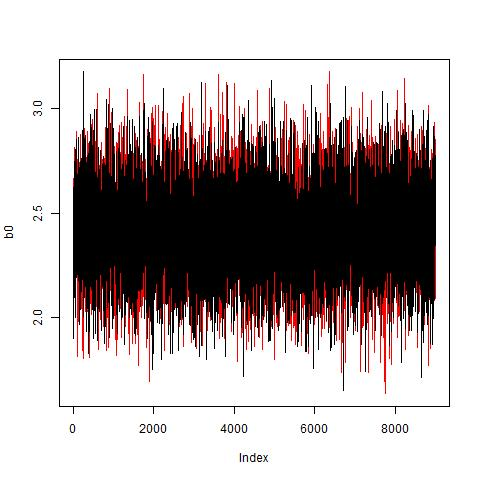
\includegraphics[width=0.35\linewidth]{Plots/tr_plot_1} }\subfloat[Traceplot for $b_1$\label{fig:unnamed-chunk-1-2}]{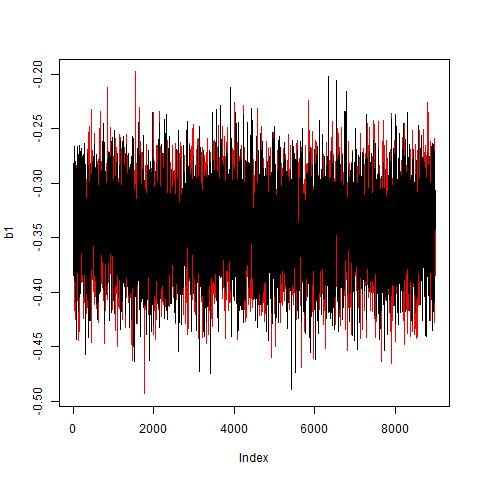
\includegraphics[width=0.35\linewidth]{Plots/tr_plot_2} }\subfloat[Traceplot for $b_2$\label{fig:unnamed-chunk-1-3}]{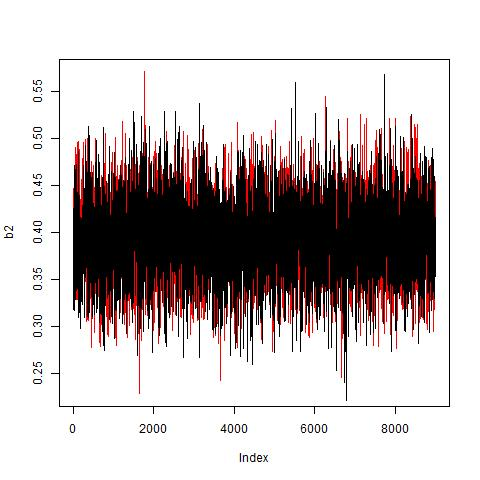
\includegraphics[width=0.35\linewidth]{Plots/tr_plot_3} }\newline\subfloat[Traceplot for $b_3$\label{fig:unnamed-chunk-1-4}]{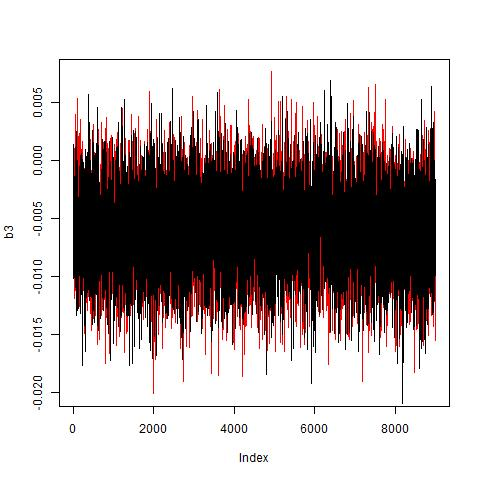
\includegraphics[width=0.35\linewidth]{Plots/tr_plot_4} }\subfloat[Traceplot for the variance\label{fig:unnamed-chunk-1-5}]{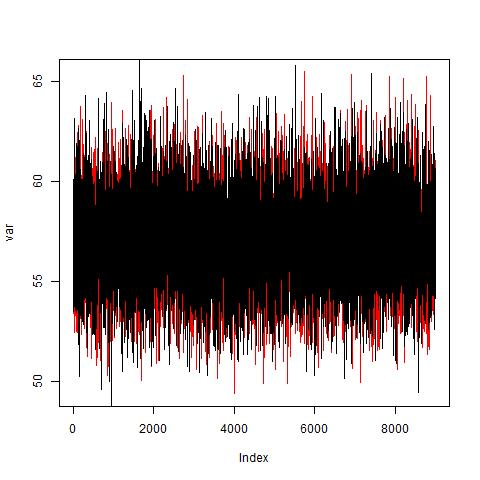
\includegraphics[width=0.35\linewidth]{Plots/tr_plot_5} }\hfill{}

\caption{Traceplots for the regression parameters}\label{fig:unnamed-chunk-1}
\end{figure}

\clearpage

\hypertarget{appendix-b-autocorrelation-plots}{%
\subsection{Appendix B: Autocorrelation
plots}\label{appendix-b-autocorrelation-plots}}

\begin{figure}

\subfloat[Autocorrelation plot for the intercept\label{fig:unnamed-chunk-2-1}]{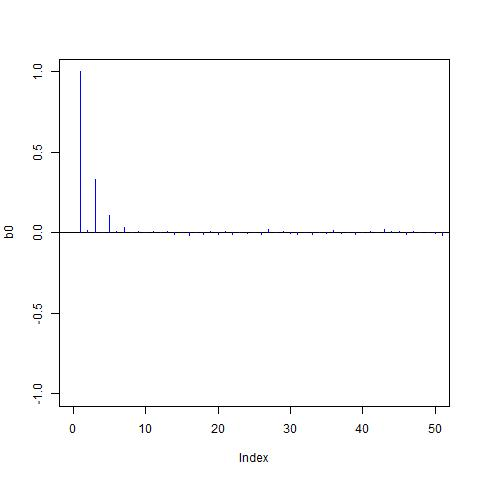
\includegraphics[width=0.35\linewidth]{Plots/acf_plot_1} }\subfloat[Autocorrelation plot for $b_1$\label{fig:unnamed-chunk-2-2}]{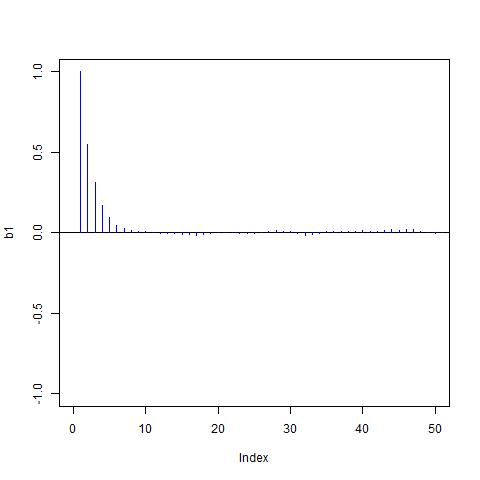
\includegraphics[width=0.35\linewidth]{Plots/acf_plot_2} }\subfloat[Autocorrelation plot for $b_2$\label{fig:unnamed-chunk-2-3}]{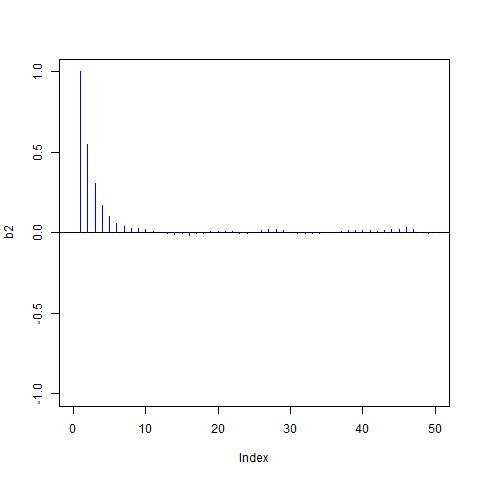
\includegraphics[width=0.35\linewidth]{Plots/acf_plot_3} }\newline\subfloat[Autocorrelation plot for $b_3$\label{fig:unnamed-chunk-2-4}]{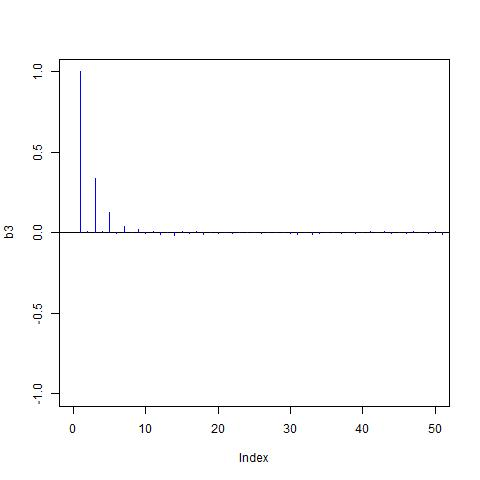
\includegraphics[width=0.35\linewidth]{Plots/acf_plot_4} }\subfloat[Autocorrelation plot for the variance\label{fig:unnamed-chunk-2-5}]{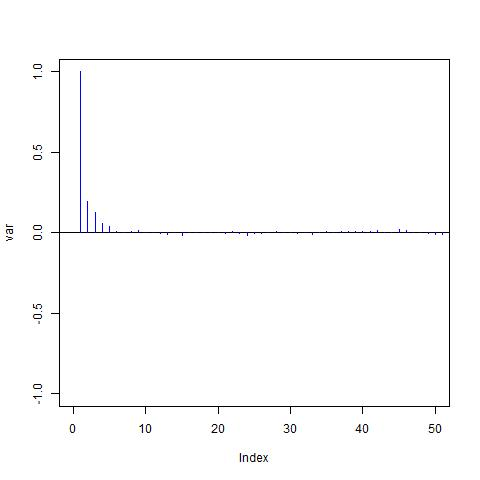
\includegraphics[width=0.35\linewidth]{Plots/acf_plot_5} }\hfill{}

\caption{Autocorrelation plots for the regression parameters}\label{fig:unnamed-chunk-2}
\end{figure}

\clearpage

\hypertarget{appendix-c-gelman-rubin-plots}{%
\subsection{Appendix C: Gelman-Rubin
plots}\label{appendix-c-gelman-rubin-plots}}

\begin{figure}

\subfloat[Gelman-Rubin plot for the intercept\label{fig:unnamed-chunk-3-1}]{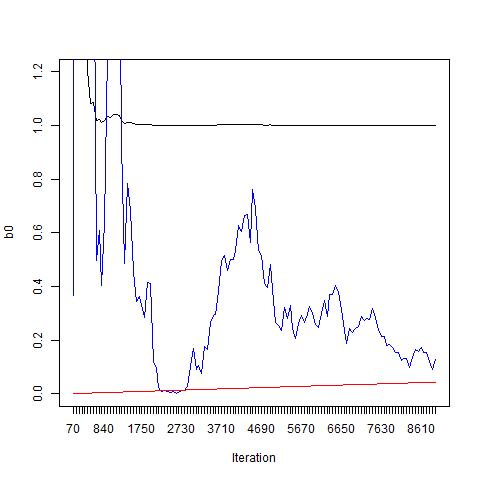
\includegraphics[width=0.35\linewidth]{Plots/gr_plot_1} }\subfloat[Gelman-Rubin plot for $b_1$\label{fig:unnamed-chunk-3-2}]{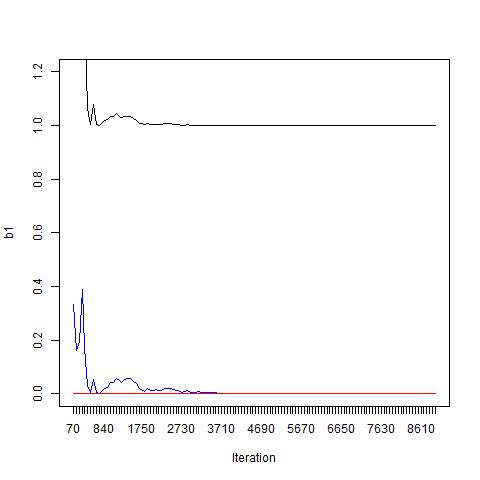
\includegraphics[width=0.35\linewidth]{Plots/gr_plot_2} }\subfloat[Gelman-Rubin plot for $b_2$\label{fig:unnamed-chunk-3-3}]{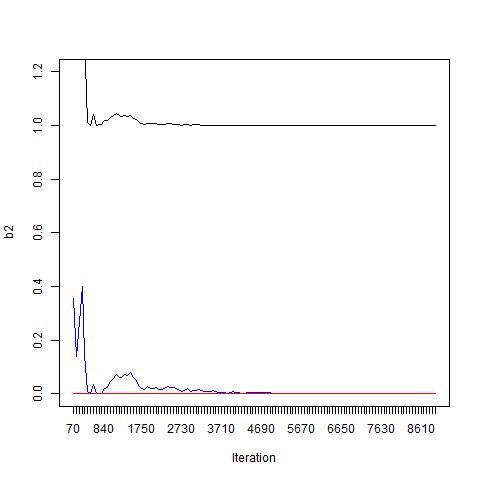
\includegraphics[width=0.35\linewidth]{Plots/gr_plot_3} }\newline\subfloat[Gelman-Rubin plot for $b_3$\label{fig:unnamed-chunk-3-4}]{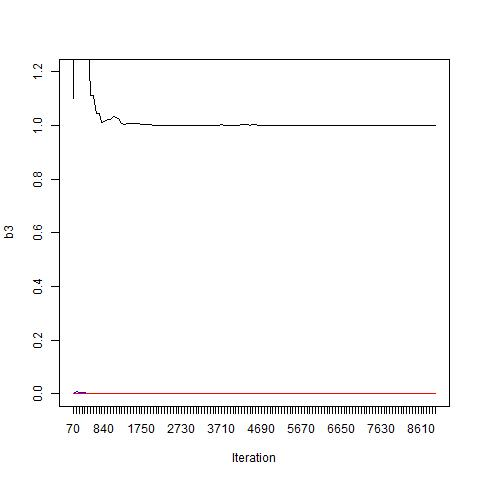
\includegraphics[width=0.35\linewidth]{Plots/gr_plot_4} }\subfloat[Gelman-Rubin plot for the variance\label{fig:unnamed-chunk-3-5}]{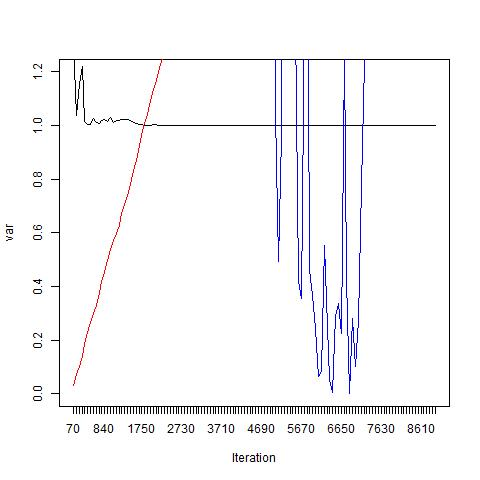
\includegraphics[width=0.35\linewidth]{Plots/gr_plot_5} }\hfill{}

\caption{Gelman-Rubin plots for the regression parameters}\label{fig:unnamed-chunk-3}
\end{figure}

\clearpage

\hypertarget{appendix-d-mcmc-errors}{%
\subsection{Appendix D: MCMC Errors}\label{appendix-d-mcmc-errors}}

\begin{longtable}[]{@{}llll@{}}
\caption{MCMC Errors for each of the regression
parameters}\tabularnewline
\toprule
Parameter & SD & MC Error & MC Error/SD \\
\midrule
\endfirsthead
\toprule
Parameter & SD & MC Error & MC Error/SD \\
\midrule
\endhead
\(b_0\) & 0.207 & 0.0021 & 0.01 \\
\(b_1\) & 0.035 & 0.0003 & 0.01 \\
\(b_2\) & 0.039 & 0.0004 & 0.01 \\
\(b_3\) & 0.004 & 0.0000 & 0.01 \\
\(var\) & 2.229 & 0.0223 & 0.01 \\
\bottomrule
\end{longtable}

\hypertarget{references}{%
\section*{References}\label{references}}
\addcontentsline{toc}{section}{References}

\hypertarget{refs}{}
\begin{CSLReferences}{1}{0}
\leavevmode\vadjust pre{\hypertarget{ref-hoijtink2019tutorial}{}}%
Hoijtink, Herbert, Joris Mulder, Caspar van Lissa, and Xin Gu. 2019.
{``A Tutorial on Testing Hypotheses Using the Bayes Factor.''}
\emph{Psychological Methods} 24 (5): 539.

\leavevmode\vadjust pre{\hypertarget{ref-nicholls1997australian}{}}%
Nicholls, Neville, Wasyl Drosdowsky, and Beth Lavery. 1997.
{``Australian Rainfall Variability and Change.''} \emph{Weather} 52 (3):
66--72.

\leavevmode\vadjust pre{\hypertarget{ref-vanbuuren2011mice}{}}%
van Buuren, Stef, and Karin Groothuis-Oudshoorn. 2011. {``{mice}:
Multivariate Imputation by Chained Equations in r.''} \emph{Journal of
Statistical Software} 45 (3): 1--67.
\url{https://doi.org/10.18637/jss.v045.i03}.

\end{CSLReferences}

\end{document}
